\documentclass{beamer}

\usepackage[T1]{fontenc}
\usepackage[utf8]{inputenc}
\usepackage[american]{babel}
\usepackage{amsmath,amssymb,amsthm}
\usepackage{tikz,pgflibraryarrows,pgflibraryplotmarks,pgflibrarysnakes,pgflibraryshapes}
\usepackage[backend=biber,citestyle=authoryear-comp,bibstyle=beamer,doi=false,isbn=false,url=false,maxnames=10]{biblatex}
\bibliography{defeo}

\mode<presentation>{%
  \usetheme{Boadilla}
}
\beamertemplatenavigationsymbolsempty

\renewcommand{\emph}[1]{{\usebeamercolor[fg]{structure}#1}}

%\let\footcite\footnote

\newcommand{\C}{\mathbb{C}}
\newcommand{\R}{\mathbb{R}}
\newcommand{\Z}{\mathbb{Z}}
\newcommand{\N}{\mathbb{N}}
\newcommand{\Q}{\mathbb{Q}}
\newcommand{\F}{\mathbb{F}}
\renewcommand{\O}{\mathcal{O}}
\newcommand{\End}{\operatorname{End}}
\newcommand{\chr}{\operatorname{char}}
\newcommand{\Cl}{\operatorname{Cl}}
\renewcommand{\a}{{\mathfrak{a}}}
\renewcommand{\b}{{\mathfrak{b}}}
\newcommand{\cyc}[1]{{\langle #1 \rangle}}
\newcommand{\ord}{\operatorname{ord}}

\usetikzlibrary{matrix,decorations,decorations.text,calc}

\pgfkeys{/triangle/.code=\tikzset{x={(-0.5cm,-0.866cm)},y={(1cm,0cm)}}}
\pgfkeys{/lattice/.code n args={4}{\tikzset{cm={#1,#2,#3,#4,(0,0)}}}}

\newcommand{\axes}[4]{
  \clip (#1,#3) rectangle (#2,#4);
  \draw [thin, gray, -latex] (#1,0) -- (#2,0);% Draw x axis
  \draw [thin, gray, -latex] (0,#3) -- (0,#4);% Draw y axis
}

\newcommand{\lattice}[2]{
  \draw[style=help lines,dashed] (#1-1,#1-1) grid[step=1] (#2+1,#2+1);
  \foreach \x in {#1,...,#2}{
    \foreach \y in {#1,...,#2}{
      \node[draw,circle,inner sep=2pt,fill] at (\x,\y) {};
      % Places a dot at those points
    }
  }
}

\newcommand{\bl}[1]{\textcolor{blue}{#1}}
\newcommand{\rd}[1]{\textcolor{red}{#1}}

% This command defines a triangle of dots of given height
\newcommand{\dottriangle}[2][\i-\j]{%
  \foreach \i in {0,...,#2} {%
    \foreach \j in {0,...,\i} {%
      \draw(\i,\j) node{#1};%
    }%
  }}


\title[Isogeny-based cryptography]{The isogeny cycle seminar}
\author{Luca De Feo}
\date[EPFL, Sep 29, 2016]{September 29, 2016, École Polytechnique Fédérale de Lausanne}
\institute[UVSQ \& INRIA]{Université de Versailles \& Inria Saclay}

\begin{document}

\frame[plain]{
  \begin{tikzpicture}[remember picture,overlay]
    \node[at=(current page.center), opacity=0.7] {
      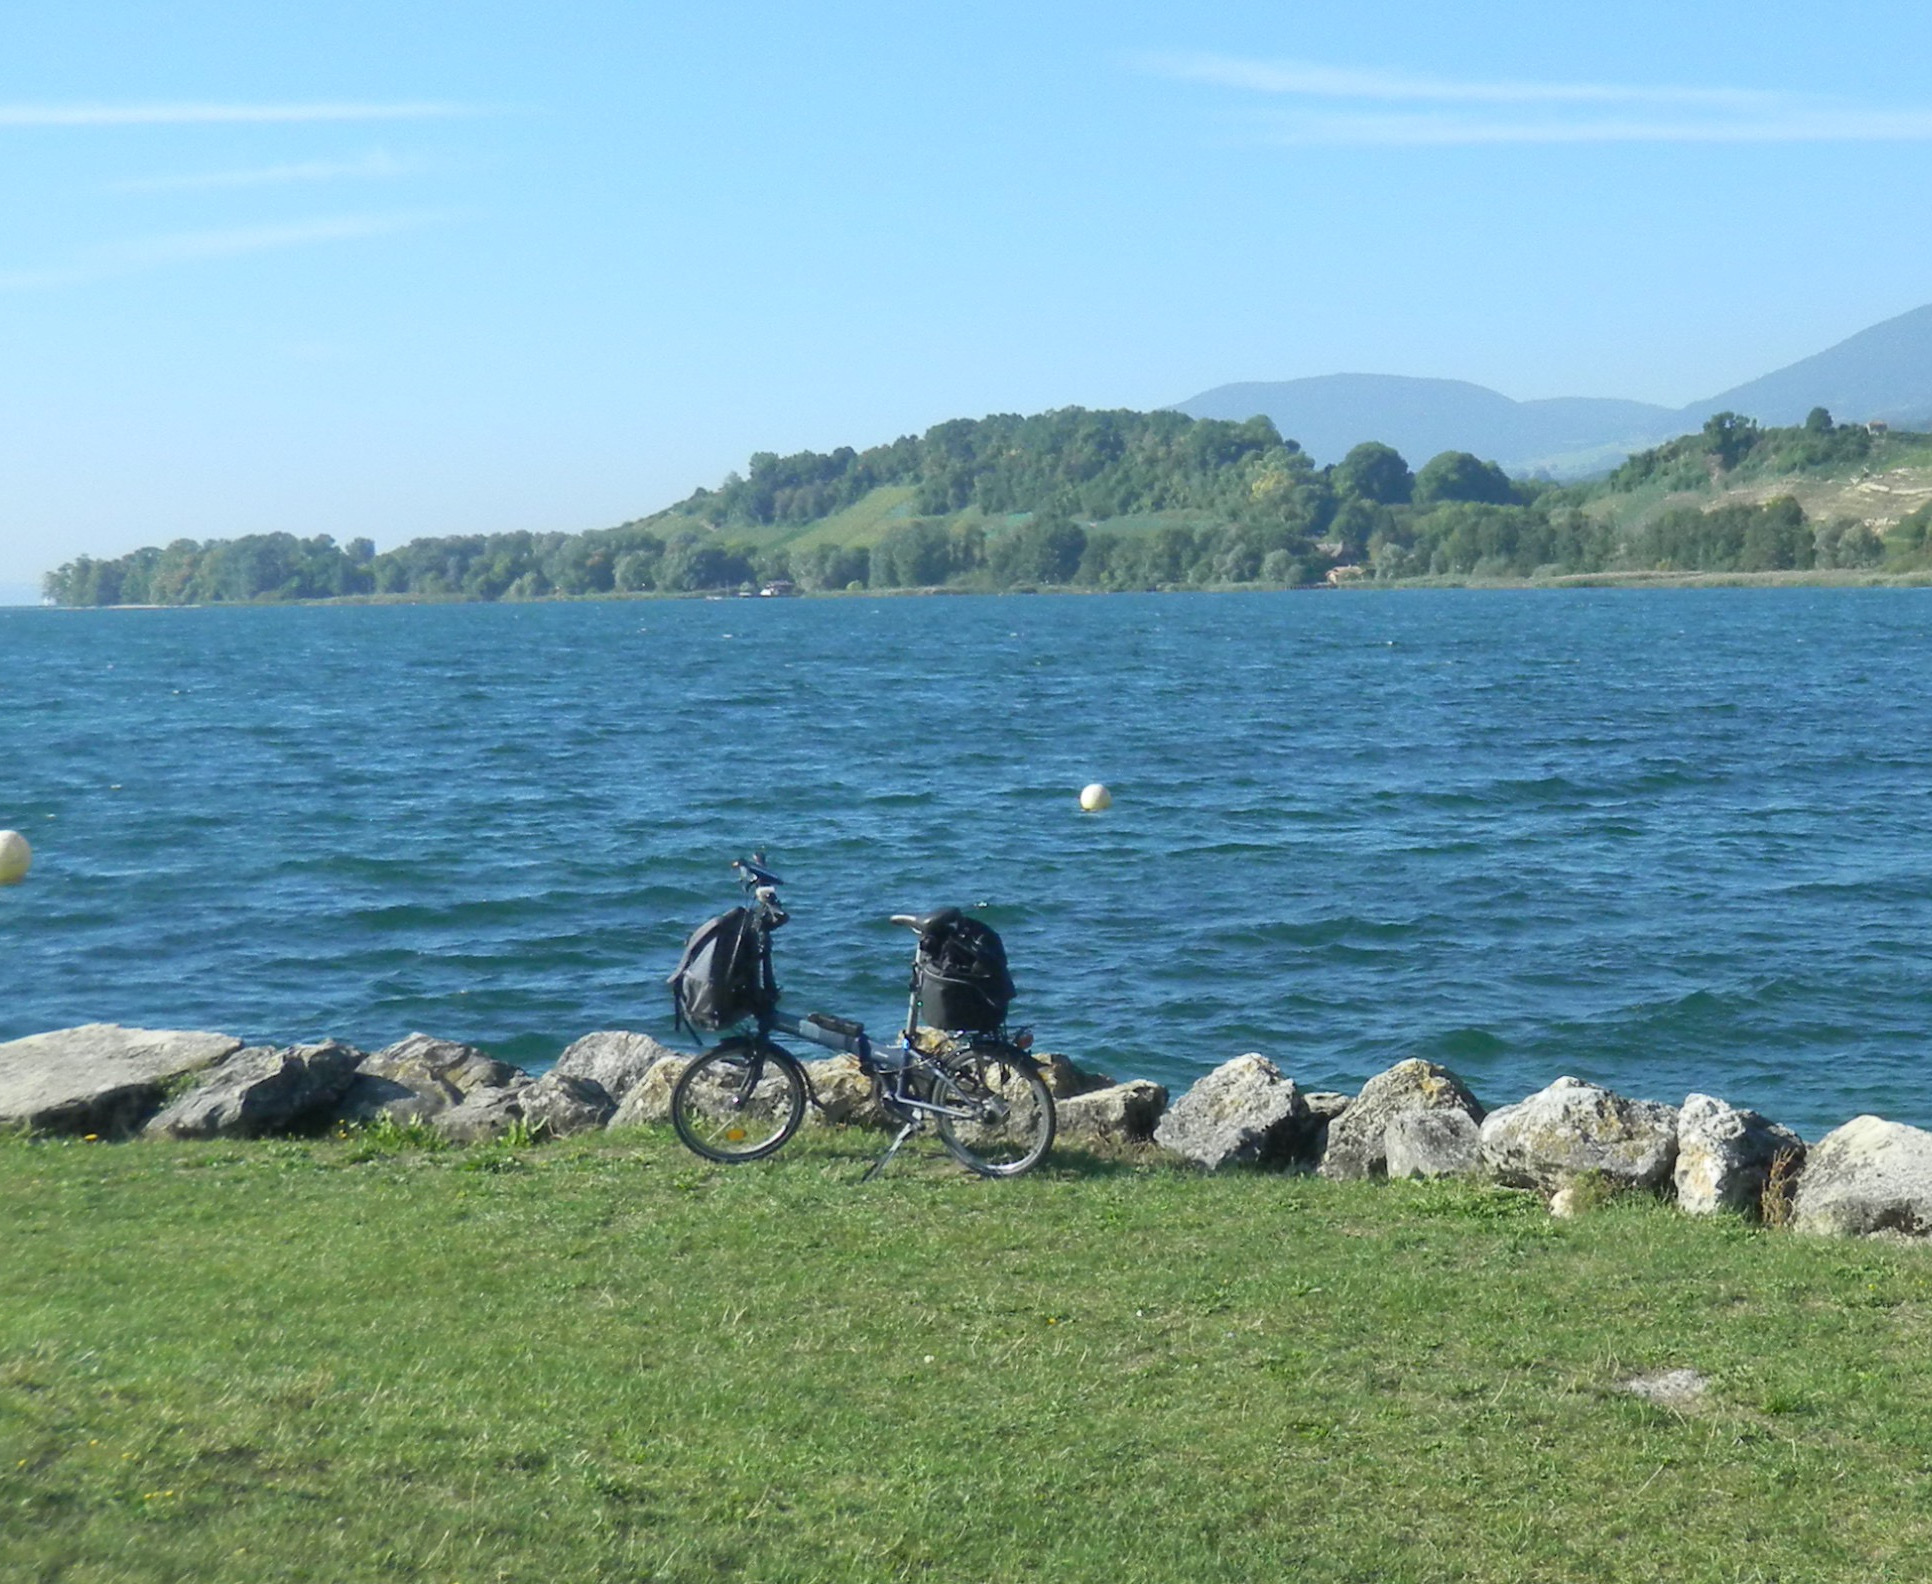
\includegraphics[width=\paperwidth]{cycle.jpg}
    };
  \end{tikzpicture}
  \vspace{-2.2cm}
  {\bf \titlepage}
}

%% 

\begin{frame}
  \frametitle{Elliptic curves}

  Let \emph{$E \;:\; y^2 = x^3 + ax + b$} be an elliptic curve\dots \uncover<2->{forget it!}

  \begin{center}
    \begin{tikzpicture}[domain=-2.4566:4,samples=100,yscale=1/2]
      \draw plot (\x,{sqrt(\x*\x*\x-4*\x+5)});
      \draw plot (\x,{-sqrt(\x*\x*\x-4*\x+5)});

      \draw[thin,gray,-latex] (0,-7) -- (0,7);
      \draw[thin,gray,-latex] (-3,0) -- (4,0);

      \draw (-3,1) -- (4,8/3+3);
      \begin{scope}[every node/.style={draw,circle,inner sep=1pt,fill},cm={1,2/3,0,0,(0,3)}]
        \node at (-2.287980,0) {};
        \node at (-0.535051,0) {};
        \node at (3.267475,0) {};
      \end{scope}
      \begin{scope}[every node/.style={yshift=0.3cm},cm={1,2/3,0,0,(0,3)}]
        \node at (-2.287980,0) {$P$};
        \node at (-0.535051,0) {$Q$};
        \node at (3.267475,0) {$R$};
      \end{scope}

      \draw[dashed] (3.267475,3.267475*2/3+3) -- (3.267475,-3.267475*2/3-3) 
      node[draw,circle,inner sep=1pt,fill] {}
      node[xshift=-0.1cm,anchor=east] {$P+Q$};

      \begin{uncoverenv}<2>
        \draw[very thick,red] (-5,-7) -- (6,7);
        \draw[very thick,red] (-5,7) -- (6,-7);
      \end{uncoverenv}
    \end{tikzpicture}
  \end{center}
\end{frame}

%%

\begin{frame}
  \frametitle{Elliptic curves}

  \begin{columns}
    \begin{column}{0.75\textwidth}
      \begin{tikzpicture}[scale=2]
        \axes{-1}{3.5}{-0.5}{3}

        \begin{scope}[/lattice={1}{0.2}{0.4}{0.7}]
          \begin{uncoverenv}<1>
            \draw[fill,black!10] (0,0) -- (1,0) -- (1,1) -- (0,1) -- (0,0);
            \node at (0.5,0.5) {$\C/\Lambda$};
            \node at (0.9,-0.1) {$\omega_1$};
            \node at (-0.1,0.9) {$\omega_2$};
          \end{uncoverenv}

          \lattice{-3}{4}

          \begin{uncoverenv}<2-5>
            \node[red] at (0.7,0.65) {$a$}; 
            \node[draw,circle,inner sep=1pt,fill,red] at (0.8,0.5) {};
            \node[red] at (0.2,0.9) {$b$}; 
            \node[draw,circle,inner sep=1pt,fill,red] at (0.3,0.7) {};
            
            \begin{uncoverenv}<3-4>
              \node[red] at (1.2,1.3) {$a+b$}; 
              \node[draw,circle,inner sep=1pt,fill,red] at (1.1,1.2) {};
              \begin{uncoverenv}<3>
                \draw[red,thin] (0,0) -- (0.8,0.5) -- (1.1,1.2);
                \draw[red,thin] (0,0) -- (0.3,0.7) -- (1.1,1.2);          
              \end{uncoverenv}
            \end{uncoverenv}

            \transdissolve<5>
            \begin{uncoverenv}<5>
              \node[red] at (0.2,0.3) {$a+b$}; 
              \node[draw,circle,inner sep=1pt,fill,red] at (0.1,0.2) {};
            \end{uncoverenv}
          \end{uncoverenv}
        \end{scope}  
      \end{tikzpicture}
    \end{column}
    \begin{column}{0.2\textwidth}
      \begin{onlyenv}<1>
        Let $\omega_1,\omega_2\in\C$ be linearly independent complex
        numbers. Set
        \[\emph{\Lambda = \omega_1\Z \oplus \omega_2\Z}\]

        $\C/\Lambda$ is an elliptic curve.
      \end{onlyenv}

      \begin{onlyenv}<2->
        Addition law induced by addition on $\mathbb{C}$.
      \end{onlyenv}
    \end{column}
  \end{columns}
\end{frame}

%%

\begin{frame}
  \frametitle{Multiplication}

  \begin{tikzpicture}[scale=2.2]
    \axes{-1}{4.5}{-0.5}{3}

    \begin{scope}[/lattice={1}{0.2}{0.4}{0.7}]
      \lattice{-3}{5}
    
      \node[red,yshift=0.2cm] at (0.8,0.6) {$a$}; 
      \draw[red] (0.8,0.6) node[fill,circle,inner sep=1pt] {};

      \begin{uncoverenv}<2>
        \node[red,yshift=0.2cm] at (2.4,1.8) {$[3]a$}; 
        \draw[red] (0,0) -- (1.6,1.2) node[fill,circle,inner sep=1pt] {} 
        -- (2.4,1.8) node[fill,circle,inner sep=1pt] {};
      \end{uncoverenv}

      \transdissolve<3>
      \begin{uncoverenv}<3>
        \node[red,yshift=0.3cm] at (0.4,0.8) {$[3]a$}; 
        \draw[red] (0.4,0.8) node[fill,circle,inner sep=1pt] {};
      \end{uncoverenv}
    \end{scope}
  \end{tikzpicture}
\end{frame}

%%

\begin{frame}
  \frametitle{Torsion subgroups}

  \begin{columns}
    \begin{column}{0.7\textwidth}
      \begin{tikzpicture}[scale=1.8]
        \axes{-0.3}{4.5}{-0.5}{4};

        \begin{scope}[/lattice={3}{0.6}{1.2}{2.1}]
          \lattice{-1}{2}

          \foreach \i in {0,...,2} {
            \foreach \j in {0,...,2} {
              \draw[red] (\i/3,\j/3) node[fill,circle,inner sep=1pt] {};
            }
          }
          \draw[red] (0,0) -- (1/3,0) node[yshift=0.2cm] {$a$};
          \draw[red] (0,0) -- (0,1/3) node[yshift=0.2cm] {$b$};
        \end{scope}
      \end{tikzpicture}  
    \end{column}
    \begin{column}{0.25\textwidth}
      The $\ell$-torsion subgroup is made up by the points
      \[\emph{\left(\frac{i\omega_1}{\ell},\frac{j\omega_2}{\ell}\right)}\]

      It is a group of rank two
      \begin{alertenv}
        \begin{align*}
          E[\ell] &= \langle a,b \rangle\\
          &\simeq (\Z/\ell\Z)^2
        \end{align*}
      \end{alertenv}
    \end{column}
  \end{columns}
\end{frame}

%%

\begin{frame}
  \frametitle{Isogenies}

  \begin{columns}
    \begin{column}{0.7\textwidth}
      \begin{tikzpicture}[scale=1.8]
        \axes{-0.3}{4.5}{-0.5}{4};
        
        \begin{scope}[/lattice={3}{0.6}{1.2}{2.1}]
          \uncover<1>{\lattice{-1}{2}}

          \begin{uncoverenv}<1-3>
            \draw[red] (0,0) -- (1/3,0) node[yshift=0.3cm] {$a$};
          \end{uncoverenv}
          \begin{uncoverenv}<4->
            \draw[red] (0,0) -- (0,1/3) node[yshift=0.3cm] {$b$};
          \end{uncoverenv}

          \begin{uncoverenv}<1-2>
            \draw[blue] (0.8,0.5) node[yshift=0.3cm] {$p$};
            \draw[blue] (0.8,0.5) node[fill,circle,inner sep=1pt] {};
          \end{uncoverenv}
        \end{scope}
        
        \begin{scope}[/lattice={1}{0.2}{1.2}{2.1}]
          \transdissolve<2>
          \uncover<2-4>{\lattice{-3}{5}}

          \transdissolve<3>
          \begin{uncoverenv}<3-5>
            \draw[blue] (0.4,0.5) node[yshift=0.3cm] {$p$};
            \draw[blue] (0.4,0.5) node[fill,circle,inner sep=1pt] {};
          \end{uncoverenv}
        \end{scope}

        \begin{scope}[/lattice={1}{0.2}{0.4}{0.7}]
          \transdissolve<5>
          \uncover<5->{\lattice{-3}{5}}

          \transdissolve<6>
          \begin{uncoverenv}<6->
            \draw[blue] (0.4,0.5) node[yshift=0.3cm] {$p$};
            \draw[blue] (0.4,0.5) node[fill,circle,inner sep=1pt] {};
          \end{uncoverenv}
        \end{scope}
        
        \begin{scope}[/lattice={3}{0.6}{1.2}{2.1}]
          \foreach \i in {0,...,2} {
            \foreach \j in {0,...,2} {
              \draw[red] (\i/3,\j/3) node[fill,circle,inner sep=1pt] {};
            }
          }
        \end{scope}
      \end{tikzpicture}  
    \end{column}
    \begin{column}{0.25\textwidth}
      \begin{onlyenv}<1-3>
        Let $\rd{a}\in\C/\Lambda_1$ be an $\ell$-torsion point, and let
        \[\emph{\Lambda_2 = a\Z\oplus\Lambda_1}\]
        Then \emph{$\Lambda_1\subset\Lambda_2$} and we define a degree
        $\ell$ cover
        \[\emph{\phi:\C/\Lambda_1\to\C/\Lambda_2}\]

        \emph{$\phi$} is a morphism of complex Lie groups and is called an
        \alert{isogeny}.
      \end{onlyenv}
      \begin{onlyenv}<4-> 
        Taking a point $\rd{b}$ not in the kernel of \emph{$\phi$}, we
        obtain a new degree $\ell$ cover
        \[\emph{\hat{\phi}:\C/\Lambda_2\to\C/\Lambda_3}\]

        The composition \emph{$\hat{\phi}\circ\phi$} has degree
        $\ell^2$ and is \alert{homothetic to the multiplication} by
        $\ell$ map.

        \emph{$\hat{\phi}$} is called the \alert{dual isogeny} of
        \emph{$\phi$}.
      \end{onlyenv}
    \end{column}
  \end{columns}
\end{frame}

%% 

\begin{frame}
  \frametitle{Isogenies over arbitrary fields}

  Isogenies are just \alert{the right notion of morphism} for elliptic
  curves

  \begin{itemize}
  \item Surjective group morphisms.
  \item Algebraic maps (i.e., defined by polynomials).
  \end{itemize}

  (Separable) isogenies $\Leftrightarrow$ finite subgroups:
  \alert{\[0 \to H \to E \overset{\phi}{\to} E' \to 0\]}
  The kernel \emph{$H$} determines the image curve \emph{$E'$} up to
  isomorphism \[\emph{E/H\overset{\text{\tiny def}}{=}E'}.\]

  \begin{block}{Isogeny degree}
    Neither of these definitions is quite correct, but they
    \textit{nearly} are:
    \begin{itemize}
    \item The degree of \emph{$\phi$} is the cardinality of \emph{$\ker\phi$}.
    \item (\emph{Bisson}) the degree of \emph{$\phi$} is the time
      needed to compute it.
    \end{itemize}
  \end{block}
\end{frame}

%%

\begin{frame}
  \frametitle{The computational point of view}
  
  \emph{In practice:} an isogeny $\phi$ is just a rational fraction (or maybe two)
  
  \alert{\[\frac{N(x)}{D(x)} = \frac{x^n + \cdots + n_1x +
      n_0}{x^{n-1} + \cdots + d_1x + d_0} \in k(x),\qquad\text{with }
    n=\deg\phi,\]}
  
  and $D(x)$ vanishes on $\ker\phi$.

  \begin{block}{The explicit isogeny problem}
    \begin{description}
    \item[Input:] A \textit{description} of the isogeny (e.g, its kernel).
    \item[Output:] The curve \emph{$E/H$} and the rational fraction \emph{$N/D$}.
    \item[Lower bound:] $\Omega(n)$.
    \end{description}
  \end{block}

  \begin{block}{The isogeny evaluation problem}
    \begin{description}
    \item[Input:] A \textit{description} of the isogeny \emph{$\phi$},
      a point \emph{$P\in E(k)$}.
    \item[Output:] The curve \emph{$E/H$} and \emph{$\phi(P)$}.
    \end{description}
  \end{block}
\end{frame}

%%

\begin{frame}
  \frametitle{Isogeny graphs}
  
  \vspace{-2mm}

  \begin{columns}
    \begin{column}{0.65\textwidth}
      We want to study the graph of elliptic curves with isogenies
      \emph{up to isomorphism}.  We say two \alert{isogenies}
      $\phi,\phi'$ are \alert{isomorphic} if:
    \end{column}
    \begin{column}{0.3\textwidth}
      \begin{center}
        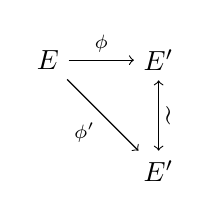
\begin{tikzpicture}[node distance=4em]
          \node(E){$E$}; 
          \node(E1)[right of=E]{$E'$};
          \node(E2)[below of=E1]{$E'$};
          \scriptsize
          \path[->] (E) edge node[auto]{$\phi$} (E1);
          \path[->] (E) edge node[auto,swap]{$\phi'$} (E2);
          \path[<->] (E1) edge node[rotate=270] {\large$\widetilde{}$} (E2);
        \end{tikzpicture}
      \end{center}
    \end{column}
  \end{columns}

  \emph{Example:} Finite field, ordinary case, graph of isogenies of degree $3$.

  \begin{center}
    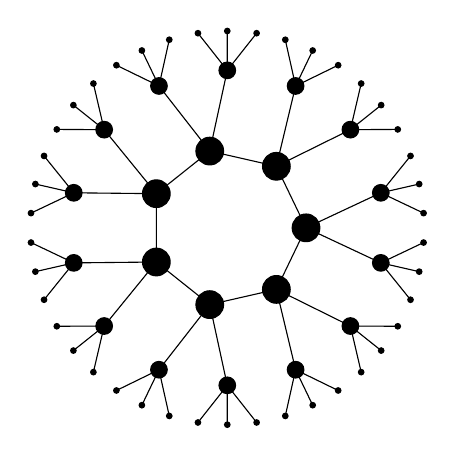
\begin{tikzpicture}[]
      \begin{scope}
        \def\crater{7}
        \foreach \i in {1,...,\crater} {
          \draw[fill] (360/\crater*\i:1cm) circle (5pt);
          \draw (360/\crater*\i : 1cm) -- (360/\crater*\i+360/\crater : 1cm);
          \foreach \j in {-1,1} {
            \draw[fill] (360/\crater*\i : 1cm) -- (360/\crater*\i + \j*360/\crater/4 : 2cm) circle (3pt);
            \foreach \k in {-1,0,1} {
              \draw[fill] (360/\crater*\i + \j*360/\crater/4 : 2cm) --
              (360/\crater*\i + + \j*360/\crater/4 + \k*360/\crater/6 : 2.5cm) circle (1pt);
            }
          }
        }
      \end{scope}
    \end{tikzpicture}
  \end{center}
\end{frame}

%%

\frame[plain]{
  \begin{tikzpicture}[remember picture,overlay]
    \node[at=(current page.center)] {
      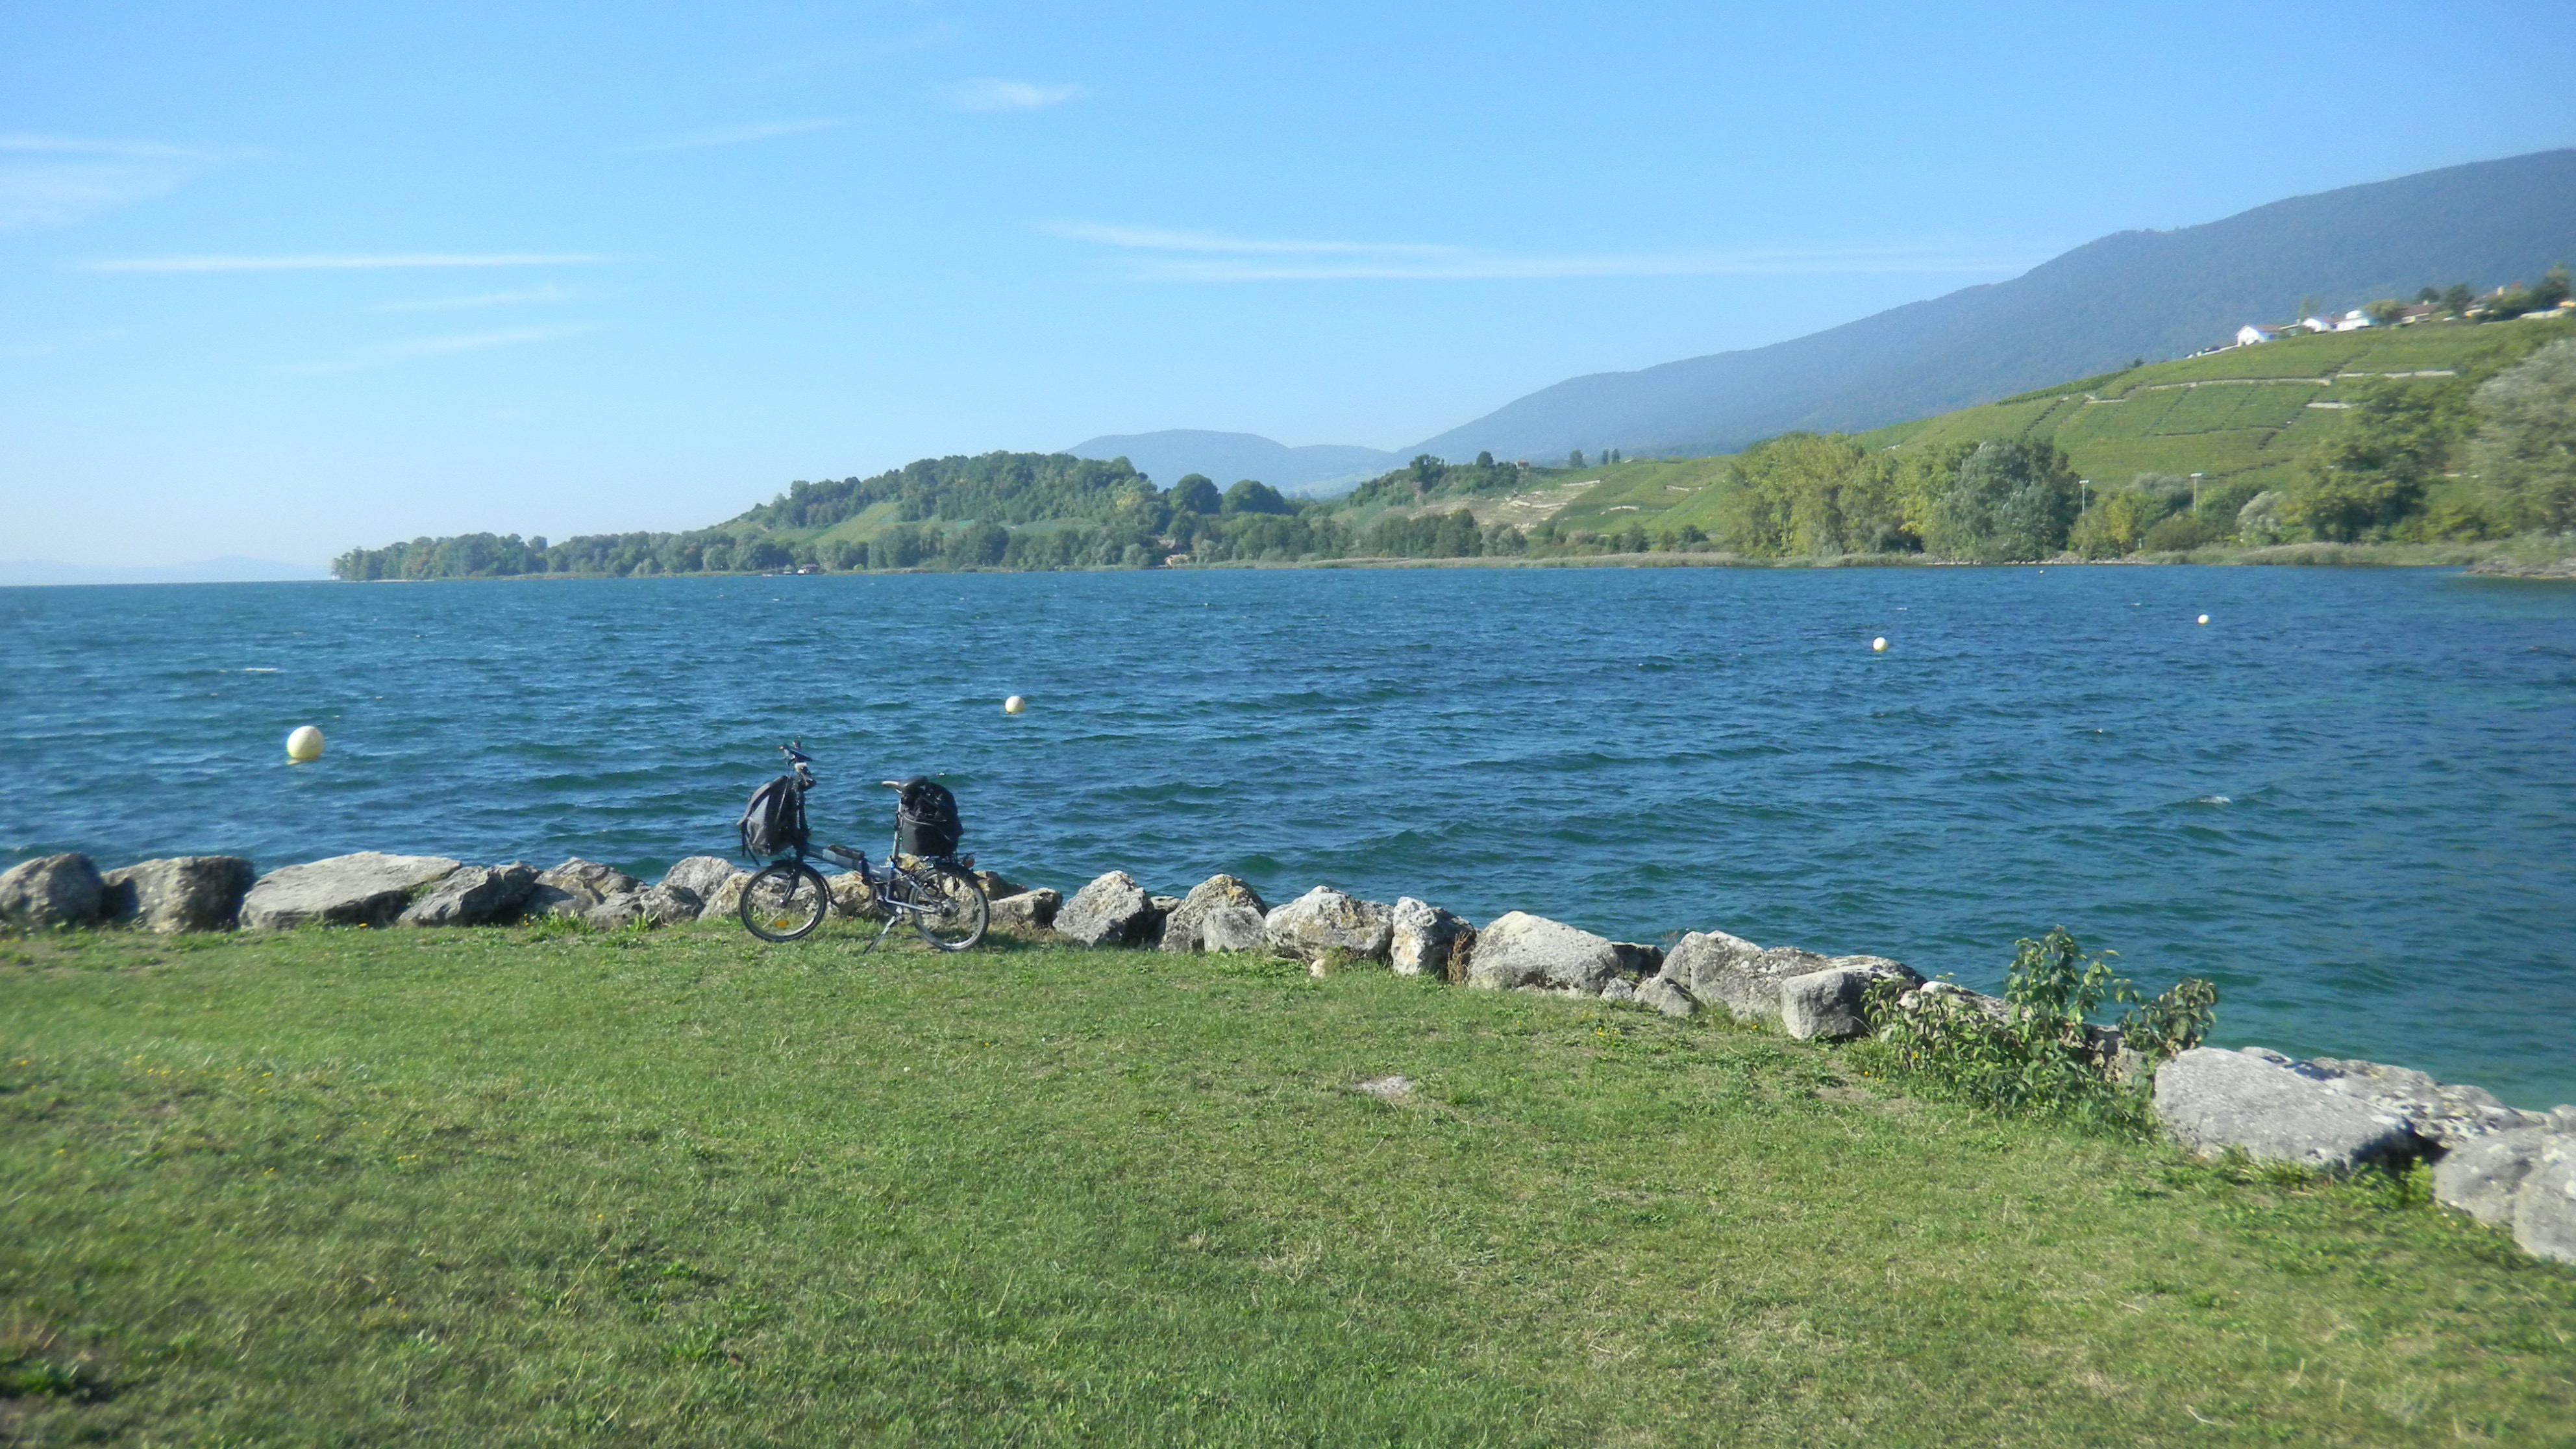
\includegraphics[height=\paperheight]{panorama.jpg}
    };
    \draw[->,very thick,blue] (current page.center) ++(-2.5,3)
    node {\Large an isogeny cycle in the Alps} ++(0,-0.2) -- ++(0,-3);
  \end{tikzpicture}
}

%%

\begin{frame}
  \frametitle{Structure of the graph\footcite{kohel,fouquet+morain02}}

  \begin{theorem}[Serre-Tate]
    Two curves are isogenous over a finite field $k$ if and only if
    they have the \alert{same number of points} on $k$.
  \end{theorem}

  \begin{block}{The graph of isogenies of \alert{prime} degree \alert{$\ell\ne p$}}
    \emph{Ordinary case}
    \begin{itemize}
    \item Nodes can have degree \emph{$0,1,2$} or \emph{$\ell+1$}.
    \item Connected components form so called \emph{volcanoes}.
    \end{itemize}
    
    \emph{Supersingular case}
    \begin{itemize}
    \item The graph is \emph{$\ell+1$-regular}.
    \item There is a \alert{unique connected component} made of all
      supersingular curves with the same number of points.
    \end{itemize}
  \end{block}
\end{frame}

%%

\begin{frame}
  \frametitle{Expander graphs}
  Let $G$ be a finite undirected $k$-regular graph.

  \begin{itemize}
  \item $k$ is the \emph{trivial eigenvalue} of the adjacency matrix
    of $G$.
  \item $G$ is called an \alert{expander} if all non-trivial
    eigenvalues satisfy \emph{$\lvert\lambda\rvert \le (1-\delta)k$}.
  \item It is called a \alert{Ramanujan graph} if
    \emph{$\lvert\lambda\rvert\le 2\sqrt{k-1}$}. This is
    \alert{optimal}.
  \end{itemize}
  
  In practice, in an expander graph \alert{random walks} of length
  \emph{$O(\frac{1}{\delta}\log\lvert G\rvert)$} land anywhere in the
  graph with probability distribution \alert{close to uniform}.

  \begin{block}{Isogeny graphs and expansion}
    \begin{itemize}
    \item The graph of \alert{ordinary isogenies} of degree less than
      \emph{$(\log 4q)^B$} is an \alert{expander} if
      \emph{$B>2$}.\footcite{jao+miller+venkatesan09}
    \item The graph of \alert{supersingular isogenies} of prime degree
      \emph{$\ell\ne p$} is
      \alert{Ramanujan}. \footcite{pizer1,pizer2}
    \end{itemize}
  \end{block}
\end{frame}

%%

\begin{frame}
  \frametitle{Isogeny walks and
    cryptanalysis\footcite{galbraith99,GHS,charles+lauter+goren09,bisson+sutherland11-rho}}
  
  \emph{Recall:} Having a \emph{weak DLP} is not isogeny invariant.

  \begin{center}
    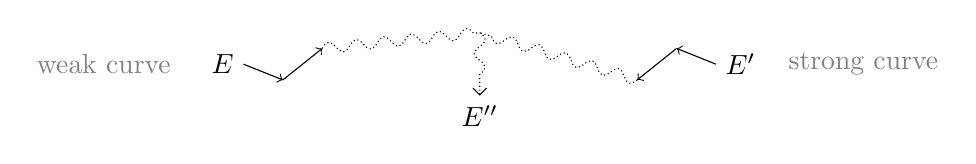
\begin{tikzpicture}
      \path (0,0) node[anchor=east] {$E$} (6,0) node[anchor=west] {$E'$};
      \path[gray] (-0.8,0) node[anchor=east] {weak curve}
      (6.8,0) node[anchor=west] {strong curve};

      \draw[->] (0,0) -- (0.5,-0.2);
      \draw[->] (6,0) -- (5.5,0.2);
      \draw[->] (0.5,-0.2) -- (1,0.2);
      \draw[->] (5.5,0.2) -- (5,-0.2);
      \begin{scope}[densely dotted,coils/.style={decorate,decoration={coil,aspect=0,amplitude=2pt}}]
        \draw[coils] (1,0.2) -- (3,0.4);
        \draw[coils] (5,-0.2) -- (3,0.4);
        \draw[-angle 90,coils] (3,0.4) -- (3, -0.4) node[anchor=north] {$E''$};
      \end{scope}
    \end{tikzpicture}
  \end{center}
  
  \begin{block}{Fourth root attacks}
    \begin{itemize}
    \item Start two random walks from the two curves and wait for a
      collision.
    \item Over \emph{$\F_q$}, the average size of an isogeny class is
      \emph{$h_\Delta\sim\sqrt{q}$}.
    \item A collision is expected after \emph{$O(\sqrt{h_\Delta}) =
        O(q^{\frac{1}{4}})$} steps.
    \end{itemize}
  \end{block}

  \emph{Note:} Can be used to build \emph{trapdoor
    systems}\footcite{teske06}.

\end{frame}

%% 

\begin{frame}
  \frametitle{Random walks and hash functions}

  Any expander graph gives rise to a hash function.

  \begin{center}
    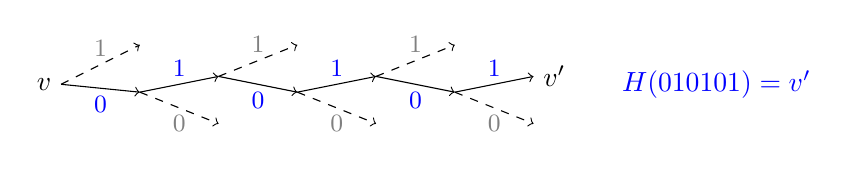
\begin{tikzpicture}
      \coordinate (last) at (0,0);
      \draw (last) node[anchor=east] {$v$};
      \foreach \i in {1,...,6} {
        \pgfmathparse{(-1)^\i}
        \let\sign\pgfmathresult
        \pgfmathparse{int(mod(\i+1,2))}
        \let\bit\pgfmathresult
        \pgfmathparse{int(mod(\i,2))}
        \let\nbit\pgfmathresult
        \draw[->] (last) -- (\i,\sign*0.1) node[blue,pos=0.5,yshift=\sign*0.2cm]{\small$\bit$};
        \draw[dashed,->] (last) -- (\i,-\sign*0.5) node[gray,pos=0.5,yshift=-\sign*0.2cm]{\small$\nbit$};
        \coordinate (last) at (\i,\sign*0.1);
      }
      \draw (last) node[anchor=west] {$v'$};

      \node[blue,anchor=west] at (7,0) {$H(010101)=v'$};
    \end{tikzpicture}
  \end{center}

  \begin{itemize}
  \item Fix a starting vertex \emph{$v$};
  \item The value to be hashed determines a random path to \emph{$v'$};
  \item \emph{$v'$} is the hash.
  \end{itemize}

  \begin{block}{Provably secure hash functions}
    \begin{itemize}
    \item Use the Ramanujan graph of \alert{supersingular
        $2$-isogenies};\footcite{charles+lauter+goren09}
    \item \alert{Collision resistance} = hardness of finding cycles in the graph;
    \item \alert{Preimage resistance} = hardness of finding a path
      from \emph{$v$} to \emph{$v'$}.
    \end{itemize}
  \end{block}
\end{frame}

%%

\begin{frame}
  \frametitle{The endomorphism ring}
  
  \begin{itemize}
  \item An \emph{endomorphism} is an isogeny \emph{$\phi:E\to E$}.
  \item The endomorphisms form a ring denoted \emph{$\End_k(E)$}.
  \end{itemize}

  \begin{theorem}
    \alert{$\Q\otimes\End_{\bar{k}}(E)$} is isomorphic to one of the
    following
    \begin{description}
    \item[ordinary case:] \alert{$\Q$} (only possible if $\chr k=0$),
    \item[ordinary case (complex multiplication):] an \alert{imaginary quadratic field},
    \item[supersingular case:] a \alert{quaternion algebra} (only possible if $\chr k\ne0$).
    \end{description}
  \end{theorem}

  \begin{corollary}
    \alert{$\End(E)$} is isomorphic to an \textit{order} 
    $\alert{\O}\subset\Q\otimes\End(E)$.
  \end{corollary}
\end{frame}

%%

\begin{frame}
  \frametitle{Isogenies and endomorphisms}

  \begin{theorem}[Serre-Tate]
    Two elliptic curves $E,E'$ are isogenous if and only if
    \[\emph{\Q\otimes\End(E) \simeq \Q\otimes\End(E')}.\]
  \end{theorem}

  \emph{Example:} Finite field, ordinary case, $3$-isogeny graph.

  \begin{center}
    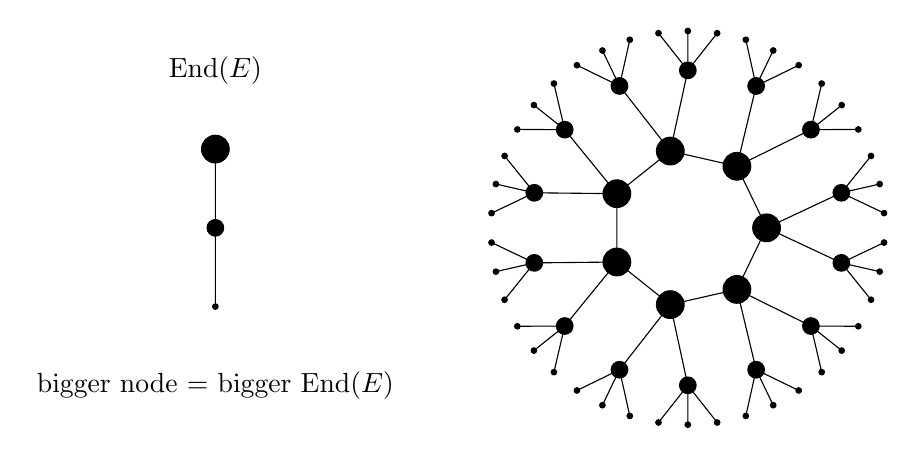
\begin{tikzpicture}[]
      \begin{scope}
        \node at (0,2) {$\End(E)$};
        \draw[fill] (0,1) circle(5pt) -- 
        (0,0) circle(3pt) --
        (0,-1) circle(1pt);
        \node at (0,-2) {bigger node = bigger $\End(E)$};
      \end{scope}
      \begin{scope}[xshift=6cm]
        \def\crater{7}
        \foreach \i in {1,...,\crater} {
          \draw[fill] (360/\crater*\i:1cm) circle (5pt);
          \draw (360/\crater*\i : 1cm) -- (360/\crater*\i+360/\crater : 1cm);
          \foreach \j in {-1,1} {
            \draw[fill] (360/\crater*\i : 1cm) -- (360/\crater*\i + \j*360/\crater/4 : 2cm) circle (3pt);
            \foreach \k in {-1,0,1} {
              \draw[fill] (360/\crater*\i + \j*360/\crater/4 : 2cm) --
              (360/\crater*\i + + \j*360/\crater/4 + \k*360/\crater/6 : 2.5cm) circle (1pt);
            }
          }
        }
      \end{scope}
    \end{tikzpicture}
  \end{center}
\end{frame}

%%

\begin{frame}
  \frametitle{The ordinary case}
  
  Let \emph{$\End(E) = \O \subset \Q(\sqrt{d})$} be the endomorphism
  ring of $E$. Define

  \begin{itemize}
  \item $\mathcal{I}(\O)$, the group of \emph{invertible fractional ideals},
  \item $\mathcal{P}(\O)$, the group of \emph{principal ideals},
  \end{itemize}
  
  \begin{definition}[The class group]
    The \alert{class group} of $\O$ is \[\alert{\Cl(\O) =
      \mathcal{I}(\O)/\mathcal{P}(O)}.\]
  \end{definition}

  \begin{itemize}
  \item It is a \alert{finite abelian} group.
  \item It arises as the Galois group of an abelian extension of
    $\Q(\sqrt{d})$.
  \item \emph{Isogeny (classes) = ideal (classes):} The class group
    acts faithfully and transitively on the isogeny graph.
  \end{itemize}
\end{frame}

%%

\begin{frame}
  \frametitle{DH-like key exchange based on (semi)-group actions}
  
  Let \emph{$G$} be an abelian group acting (faithfully and
  transitively) on a set $\emph{X}$.

  \begin{center}
    \begin{tikzpicture}
      \Large
      \node[matrix of math nodes, ampersand replacement=\&, column sep=0cm, row sep=1cm] (diagram) {
        \& |(1)| x_0 \\
        |(a)| g\cdot x_0 \& \& |(b)| h\cdot x_0\\
        \& |(ab)| gh\cdot x_0 = hg\cdot x_0\\
      };
      \small
      \path[->] (1) edge node[auto,swap]{$g$} (a);
      \path[->] (1) edge node[auto]{$h$} (b);
      \path[->] (a) edge node[auto,swap]{$h$} (ab);
      \path[->] (b) edge node[auto]{$g$} (ab);
    \end{tikzpicture}
  \end{center}
\end{frame}

%%

\begin{frame}
  \frametitle{Hidden Subgroup Problem}

  Let \emph{$G$} be a group, \emph{$X$} a set and \emph{$f:G\to X$}.
  We say that $f$ \emph{hides} a subgroup \emph{$H\subset G$} if
  \[\alert{f(g_1) = f(g_2) \Leftrightarrow g_1H = g_2H}.\]

  \begin{definition}[Hidden Subgroup Problem (HSP)]
    \begin{description}
    \item[Input:] $G,X$ as above,  an oracle computing $f$.
    \item[Output:] generators of $H$.
    \end{description}
  \end{definition}

  \begin{theorem}[Schorr, Josza]
    If $G$ is abelian, then
    \begin{itemize}
    \item \alert{$\text{HSP}\in\text{poly}_\text{BQP}(\log|G|)$},
    \item using \alert{$\text{poly}(\log|G|)$} queries to the oracle.
    \end{itemize}
  \end{theorem}
\end{frame}

%%

\begin{frame}
  \frametitle{Post-Quantum cryptography}

  \begin{block}{Known reductions}
    \begin{itemize}
    \item \alert{Discrete Log} on $\alert{G}$ of size $\alert{p} \to$
      \alert{HSP} on \alert{$(\Z/p\Z)^2$},
    \item hence DH, ECDH, etc. are broken by quantum computers.
    \item \alert{Semigroup-DH} on $\alert{G} \to$ \alert{HSP} on the
      \alert{dihedral group $G\ltimes\Z/2\Z$}.
    \end{itemize}
  \end{block}

  \begin{block}{Quantum algorithms for dihedral HSP}
    \begin{description}
    \item[Kuperberg\footcite{Kup}:] \alert{$2^{O(\sqrt{\log|G|})}$}
      quantum time, space and query complexity.
    \item[Regev\footcite{regev04}:]
      \alert{$L_{|G|}(\frac{1}{2},\sqrt{2})$} quantum time and query
      complexity, \alert{$\text{poly}(\log(|G|)$} quantum space.
    \end{description}
  \end{block}
  
  \emph{Remark (Regev):} certain lattice-based cryptosystems are also
  vulnerable to the HSP for dihedral groups.
\end{frame}

%%

\begin{frame}
  \frametitle{DH using class groups\footcite{R&S}}
  
  \emph{Public data:}
  \begin{itemize}
  \item \alert{$E/\F_p$ ordinary elliptic curve} with complex multiplication
    field $\mathbb{K}$,
  \item primes \bl{$\ell_1$},\rd{$\ell_2$}
    not dividing $\mathrm{Disc}(E)$ and
    s.t. $\left(\frac{D_\mathbb{K}}{\ell_i}\right)=1$.
  \item A \textit{direction} on the isogeny graph (i.e.\ an element of the class group).
  \end{itemize}

  \emph{Secret data:}  \alert{Random walks $\a,\b$} in the
  $\ell_i$-isogeny graphs.
  
  \begin{center}
    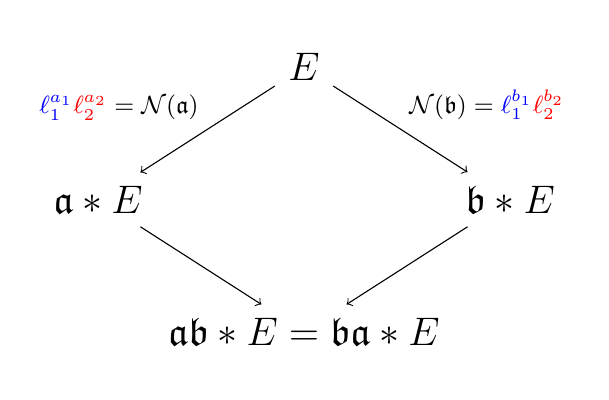
\begin{tikzpicture}
      \Large
      \node[matrix of math nodes, ampersand replacement=\&, column sep=0cm, row sep=1cm] (diagram) {
        \& |(1)| E \\
        |(a)| \a\ast E \& \& |(b)| \b\ast E\\
        \& |(ab)| \a\b\ast E = \b\a\ast E\\
      };
      \small
      \path[->] (1) edge node[auto,swap]{$\bl{\ell_1^{a_1}}\rd{\ell_2^{a_2}}=\mathcal{N}(\a)$} (a);
      \path[->] (1) edge node[auto]{$\mathcal{N}(\b)=\bl{\ell_1^{b_1}}\rd{\ell_2^{b_2}}$} (b);
      \path[->] (a) edge (ab);
      \path[->] (b) edge (ab);
    \end{tikzpicture}
  \end{center}
\end{frame}

%%

\begin{frame}
  \frametitle{R\&S key exchange}

  \begin{center}
    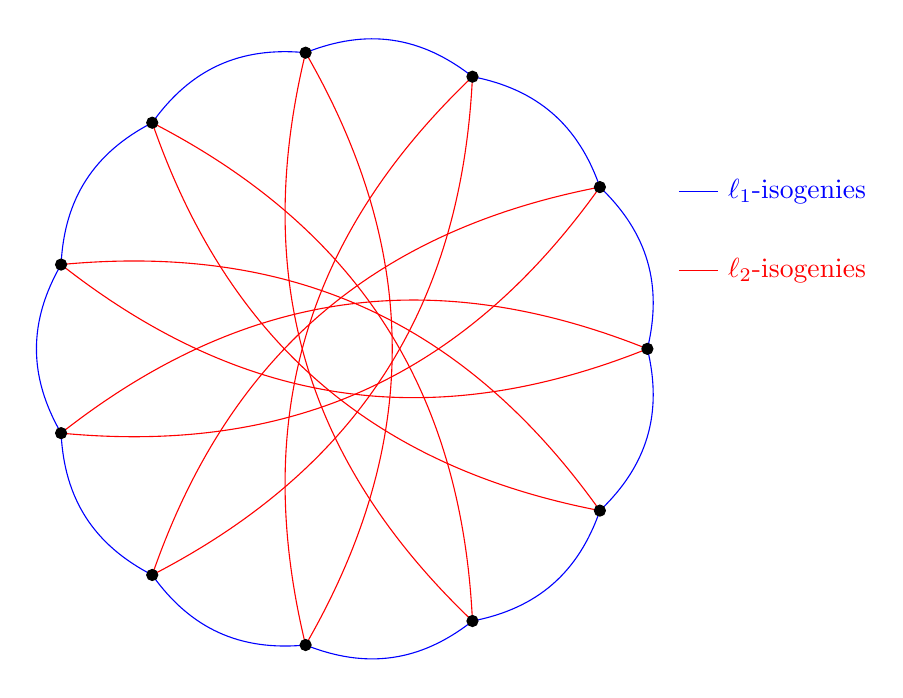
\begin{tikzpicture}
      \begin{scope}
        \def\crater{11}
        \def\jump{5}
        \def\diam{3.8cm}

        \foreach \i in {1,...,\crater} {
          \draw[blue] (360/\crater*\i : \diam) to[bend right] (360/\crater*\i+360/\crater : \diam);
          \draw[red] (360/\crater*\i : \diam) to[bend left] (360/\crater*\i+\jump*360/\crater : \diam);
        }
        \foreach \i in {1,...,\crater}
          \draw[fill] (360/\crater*\i: \diam) circle (2pt);
      \end{scope}
      \begin{scope}[xshift=4.2cm, yshift=2cm]
        \draw[blue] (0,0) -- (0.5,0) (0.5,0) node[anchor=west] {\bl{$\ell_1$}-isogenies};
        \draw[red] (0,-1) -- (0.5,-1) (0.5,-1) node[anchor=west] {\rd{$\ell_2$}-isogenies};
      \end{scope}
    \end{tikzpicture}
  \end{center}
\end{frame}

%%

\begin{frame}
  \frametitle{R\&S key exchange}

  \begin{center}
    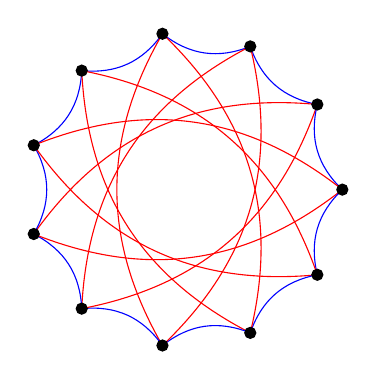
\begin{tikzpicture}
      \begin{scope}
        \def\crater{11}
        \def\jump{5}
        \def\diam{2cm}

        \foreach \i in {1,...,\crater} {
          \draw[blue] (360/\crater*\i : \diam) to[bend left] (360/\crater*\i+360/\crater : \diam);
          \draw[red] (360/\crater*\i : \diam) to[bend right] (360/\crater*\i+\jump*360/\crater : \diam);
        }
        \foreach \i in {1,...,\crater}
          \draw[fill] (360/\crater*\i: \diam) circle (2pt);
      \end{scope}
    \end{tikzpicture}
  \end{center}

  \begin{description}
  \item[Key generation:] compose small degree
    isogenies\\\alert{polynomial in the lenght of the random walk}.
  \item[Attack:] find an isogeny between two curves\\\alert{polynomial
      in the degree, exponential in the length}.
  \item[Quantum\footcite{childs+jao+soukharev10}:] HShP + isogeny
    evaluation\\\alert{subexponential in the length of the walk}.
  \end{description}
\end{frame}

%%

\begin{frame}
  \frametitle{Supersingular curves}

  \emph{$\Q\otimes\End(E)$} is a quaternion algebra (non-commutative)

  \begin{block}{Facts}
    \begin{itemize}
    \item Every supersingular curve is defined over \alert{$\F_{p^2}$}.
    \item $\alert{E(\F_{p^2}) \simeq (\Z/(p+1)\Z)^2}\;$ (up to twist, and overly simplifying!).
    \item There are $g(X_0(p))+1 \sim\alert{\frac{p+1}{12}}$ supersingular curves
      up to isomorphism.
    \item For every \emph{maximal order type} of the quaternion
      algebra $\Q_{p,\infty}$ there are \emph{$1$ or $2$ curves over
        $\F_{p^2}$} having endomorphism ring isomorphic to it.
    \item There is a \alert{unique isogeny class} of supersingular
      curves over $\bar{\F}_p$ (there are two over any finite field).
    \item The graph of \emph{$\ell$}-isogenies is
      \emph{$\ell+1$}-regular.
    \end{itemize}
  \end{block}
\end{frame}

%%

\begin{frame}
  \frametitle{R\&S key exchange with supersingular curves}
  
  \begin{description}
  \item[Good news:] there is no action of a commutative class group.
  \item[Bad news:] there is no action of a commutative class group.
  \end{description}

  \alert{However:} left ideals of \emph{$\End(E)$} still act on the isogeny graph:

  \begin{center}
    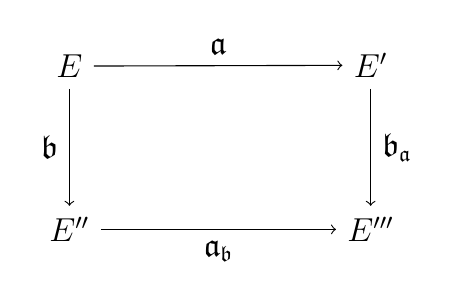
\begin{tikzpicture}
      \large
      \node[matrix of nodes, ampersand replacement=\&, column sep=3cm, row sep=1.5cm] (diagram) {
        |(E)| $E$ \& |(Es)| $E'$ \\
        |(Ep)| {$E''$} \& |(Eps)| {$E'''$}\\
      };
      \path[->] (E) edge node[auto] {$\a$} (Es);
      \path[->] (Ep) edge node[auto,swap] {$\a_\b$} (Eps);
      \path[->] (E) edge node[auto,swap] {$\b$} (Ep);
      \path[->] (Es) edge node[auto] {$\b_\a$} (Eps);
    \end{tikzpicture}
  \end{center}

  \begin{itemize}
  \item The action factors through the \emph{right-isomorphism}
    equivalence of ideals.
  \item Ideal classes form a \emph{groupoid} (in other words, an
    undirected multigraph\dots).
  \end{itemize}
\end{frame}

%%

\begin{frame}
  \frametitle{From ideals back to isogenies}

  In practice, computations with ideals are hard. We fix, instead:

  \begin{itemize}
  \item Small primes \bl{$\ell_A$}, \rd{$\ell_B$};
  \item A large prime \emph{$p$} such that $p+1 =
    \bl{\ell_A^{e_A}}\rd{\ell_B^{e_B}}$;
  \item A supersingular curve \emph{$E$} over \emph{$\F_{p^2}$}, such that
    \[E \simeq (\Z/(p+1)\Z)^2 = \bl{(\Z/\ell_A^{e_A}\Z)^2} \oplus \rd{(\Z/\ell_B^{e_B}\Z)^2},\]
  \item We use isogenies of degrees \bl{$\ell_A^{e_A}$} and
    \rd{$\ell_B^{e_B}$} with \emph{cyclic rational kernels};
  \item The diagram below can be constructed in time
    $\text{poly}(\bl{e_A}+\rd{e_B})$.
  \end{itemize}

  \begin{center}
    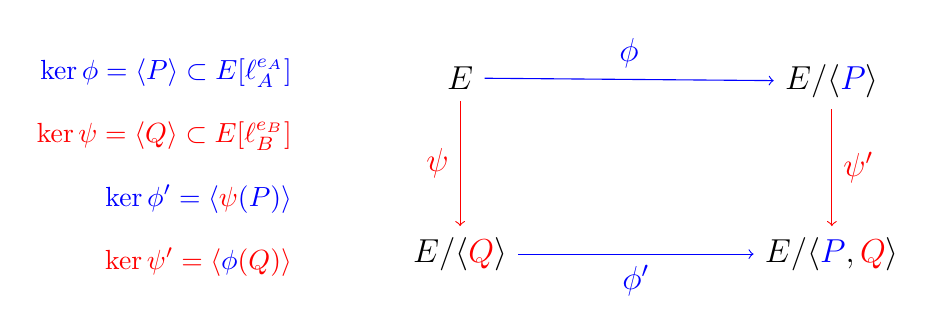
\begin{tikzpicture}
      \begin{scope}
        \draw (0,1.2) node[anchor=east,blue] {$\ker\phi=\cyc{P}\subset E[\ell_A^{e_A}]$};
        \draw (0,0.4) node[anchor=east,red] {$\ker\psi=\cyc{Q}\subset E[\ell_B^{e_B}]$};
        \draw (0,-0.4) node[anchor=east,blue] {$\ker\phi' = \cyc{\rd{\psi}(P)}$};
        \draw (0,-1.2) node[anchor=east,red] {$\ker\psi' = \cyc{\bl{\phi}(Q)}$};
      \end{scope}
      \begin{scope}[xshift=4.5cm]
        \large
        \node[matrix of nodes, ampersand replacement=\&, column sep=3cm, row sep=1.5cm] (diagram) {
          |(E)| $E$ \& |(Es)| $E/\cyc{\bl{P}}$ \\
          |(Ep)| {$E/\cyc{\rd{Q}}$} \& |(Eps)| {$E/\cyc{\bl{P},\rd{Q}}$}\\
        };
        \path[->,blue] (E) edge node[auto] {$\phi$} (Es);
        \path[->,blue] (Ep) edge node[auto,swap] {$\phi'$} (Eps);
        \path[->,red] (E) edge node[auto,swap] {$\psi$} (Ep);
        \path[->,red] (Es) edge node[auto] {$\psi'$} (Eps);
      \end{scope}
    \end{tikzpicture}
  \end{center}
\end{frame}

%%

\begin{frame}
  \frametitle{Our proposal: SIDH\footcite{jao+defeo2011}}

  \vspace{-1cm}

  \begin{columns}
    \begin{column}{0.4\textwidth}
      \begin{block}{}
        \emph{Public data:}
        \begin{itemize}
          \setlength{\itemsep}{1.5ex}
        \item Prime $p$ such that $p+1 = \bl{\ell_A^a}\rd{\ell_B^b}$;
        \item Supersingular curve \emph{$E\simeq (\Z/(p+1)\Z)^2$};
        \item \bl{$E[\ell_A^a] = \cyc{P_A,Q_A}$};
        \item \rd{$E[\ell_B^b] = \cyc{P_B,Q_B}$}.
        \end{itemize}

        \emph{Secret data:}
        \begin{itemize}
          \setlength{\itemsep}{1.5ex}
        \item \bl{$R_A = m_AP_A + n_AQ_A$},
        \item \rd{$R_B = m_BP_B + n_BQ_B$},
        \end{itemize}
      \end{block}
    \end{column}
    \begin{column}{0.58\textwidth}
      \begin{center}
        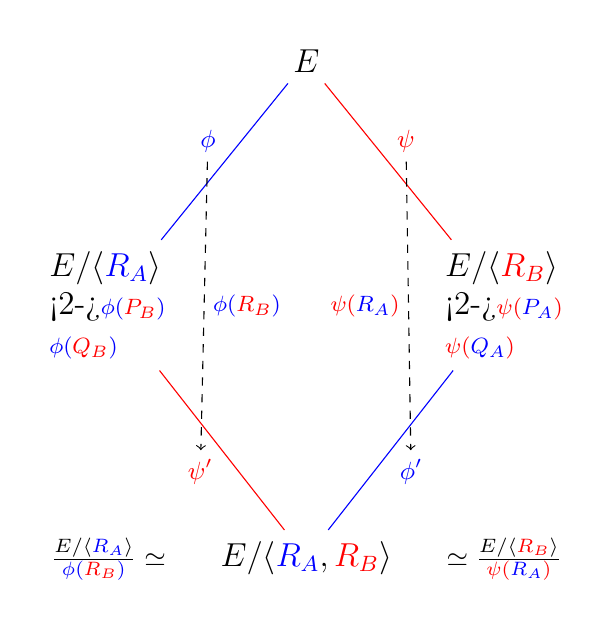
\begin{tikzpicture}
          \large
          \node[matrix of nodes, ampersand replacement=\&, column sep=4mm, row sep=2cm] (diagram) {
            \& |(1)| $E$ \\
            |(a)| \parbox{1.5cm}{$E/\cyc{\bl{R_A}}$\\\uncover<2->{{\footnotesize $\bl{\phi(}\rd{P_B}\bl{)}\\\bl{\phi(}\rd{Q_B}\bl{)}$}}} \& \&
            |(b)| \parbox{1.5cm}{$E/\cyc{\rd{R_B}}$\\\uncover<2->{{\footnotesize $\rd{\psi(}\bl{P_A}\rd{)}\\\rd{\psi(}\bl{Q_A}\rd{)}$}}}\\
            \normalsize $\frac{E/\cyc{\bl{R_A}}}{\alert{\bl{\phi(}\rd{R_B}\bl{)}}} \simeq$ \&
            |(ab)|  $E/\cyc{\bl{R_A},\rd{R_B}}$ \&
            \normalsize $\simeq \frac{E/\cyc{\rd{R_B}}}{\alert{\rd{\psi(}\bl{R_A}\rd{)}}}$\\
          };
          \small
          \path[blue] (1) edge node[auto,swap](phia) {$\phi$} (a);
          \path[red] (1) edge node[auto](phib) {$\psi$} (b);
          \path[red] (a) edge node[auto,swap](psia){$\psi'$} (ab);
          \path[blue] (b) edge node[auto](psib){$\phi'$} (ab);
          \uncover<3>{\path[dashed,->] (phia) edge node[auto]{\footnotesize $\bl{\phi(}\rd{R_B}\bl{)}$} (psia);}
          \uncover<3>{\path[dashed,->] (phib) edge node[auto,swap]{\footnotesize $\rd{\psi(}\bl{R_A}\rd{)}$} (psib);}
        \end{tikzpicture}
      \end{center}  
    \end{column}
  \end{columns}
\end{frame}

%%

\begin{frame}
  \frametitle{Other protocols based on SIDH}

  \begin{block}{Non-interactive protocols}
    \begin{itemize}
    \item El-Gamal encryption.
    \end{itemize}
  \end{block}
  
  \begin{block}{Interactive protocols}
    \begin{itemize}
    \item Zero-knowledge proofs of identity\footcite{defeo+jao+plut12},
    \item Undeniable signatures\footcite{jao2014isogeny},
    \item Strong designated verifier signatures\footcite{sun2012toward},
    \item Authenticated encryption\footcite{soukharev2016post}.
    \end{itemize}
  \end{block}

  \alert{Missing:} Classical signatures, \dots
\end{frame}

%%

\begin{frame}
  \frametitle{Generic attacks}
  
  \emph{Problem:} Given \emph{$E,E'$}, isogenous of degree
  \emph{$\ell^n$}, find \emph{$\phi:E\to E'$}.

  \begin{center}
    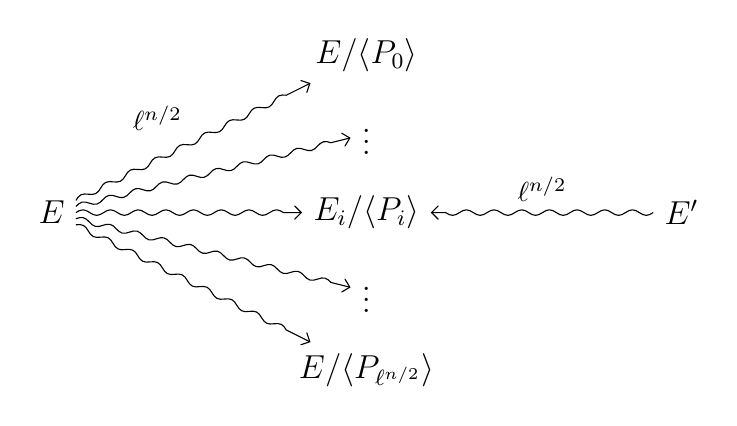
\begin{tikzpicture}[xscale=4,coils/.style={-angle 90,decorate,decoration={coil,aspect=0,amplitude=1pt}}]
      \large
      \draw (0,2) node(E) {$E$};

      \draw (1,4) node(E1) {$E/\cyc{P_0}$};
      \draw (1,2) node(Ei) {$E_i/\cyc{P_i}$};
      \draw (1,0) node(En) {$E/\cyc{P_{\ell^{n/2}}}$};
      \draw (1,3) node(dots1) {$\vdots$};
      \draw (1,1) node(dots2) {$\vdots$};

      \draw (2,2) node(E') {$E'$};

      \draw (E) edge[coils] node[auto] {\normalsize$\ell^{n/2}$} (E1);
      \draw (E) edge[coils] (Ei);
      \draw (E) edge[coils] (En);
      \draw (E) edge[coils] (dots1);
      \draw (E) edge[coils] (dots2);

      \draw (E') edge[coils] node[auto,swap] {\normalsize$\ell^{n/2}$} (Ei);
    \end{tikzpicture}
  \end{center}

  \begin{itemize}
  \item With high probability $\phi$ is the unique collision (or \textit{claw}).
  \item A \emph{quantum claw finding}\footcite{tani08} algorithm solves
    the problem in $\alert{O(\ell^{n/3})}$.
  \end{itemize}
\end{frame}

%%

\begin{frame}
  \frametitle{Other attacks}

  \begin{block}{Ephemeral key recovery (total break)}
    Given $E_0$ and a public curve $E_0/\cyc{R}$, find
    the kernel of the secret isogeny:
    \begin{description}
    \item[Subexponential] $L_p(1/2, \sqrt{3}/2)$ 
      when both curves are defined over $\F_p$.\footcite{biasse2014quantum}
    \item[Polynomial] isomorphic problem
      on quaternion algebras.\footcite{kohel2014quaternion}
    \item[Equivalent to] computing the endomorphism rings of both $E_0$
      and $E_0/\cyc{R_A}$.\footcite{galbraithsecurity}
    \end{description}
  \end{block}
\end{frame}

%%

\begin{frame}
  \frametitle{Other attacks}

  \begin{block}{Other security models}
    \renewcommand{\thefootnote}{\alph{footnote}}
    \begin{description}
    \item[Active attack] against long term keys, learns the full key
      with (close to) optimal number of oracle
      queries. Countermeasures are relatively
      expensive.\footcite{galbraithsecurity}
    \item[Side channel] Constant-time implementation
      available.\footcite{costello2015four}
    \item[] Attack on partially leaked
      keys.\footnotemark[1]
    \end{description}
  \end{block}


\end{frame}

%% 

\begin{frame}
  \frametitle{Recommended parameters}
  
  \begin{itemize}
  \item For efficiency chose $p$ such that \alert{$p+1 = 2^a3^b$}.
  \item For classical $n$-bit security, choose \alert{$2^a\sim3^b\sim2^{2n}$}, hence \alert{$p\sim2^{4n}$}.
  \item For quantum $n$-bit security, choose \alert{$2^a\sim3^b\sim2^{3n}$}, hence \alert{$p\sim2^{6n}$}.
  \end{itemize}

  \begin{block}{Practical optimizations:}
    \renewcommand{\thefootnote}{\alph{footnote}}
    \begin{itemize}
    \item Optimize arithmetic for $\F_p$.\footcite{costello2015four}\footcite{vercauteren-sidh-fp}
    \item $-1$ is a quadratic non-residue: \alert{$\F_{p^2}\simeq\F_p[X]/(X^2+1)$}.
    \item $E$ (or its twist) has a $4$-torsion point: use \alert{Montgomery} form.
    \item Avoid inversions by using \textit{projective curve
        equations}.\footnotemark[1]
    \item Use $j=0$ as starting curve.\footnotemark[1]
    \end{itemize}

    Fastest implementation\footnotemark[1]: \emph{100Mcycles} (Intel
    Haswell) \emph{@128bits} quantum security level, \emph{4512bits}
    public key size.
  \end{block}
\end{frame}

%%

\begin{frame}
  \frametitle{Evaluating $\phi:E\to E/\cyc{R}$ efficiently}
  
  \alert{$\ord(R)=\ell^a$} and \alert{$\phi = \phi_0 \circ \phi_1 \circ \cdots
    \circ \phi_{a-1}$}, each of degree $\alert{\ell}$

  \begin{center}
  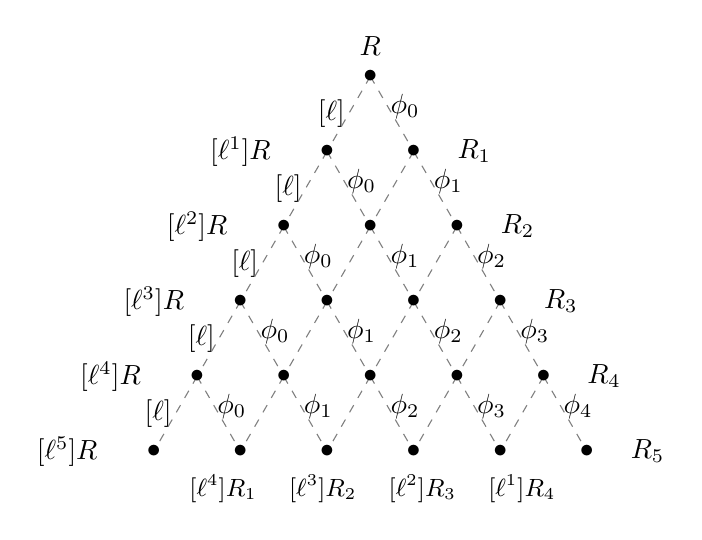
\begin{tikzpicture}[/triangle,scale=1.1]
    \def\n{5}
    \pgfmathtruncatemacro{\pn}{\n-1}
    

    \draw(-0.4,-0.2) node{$R$};

    \foreach \i in {1,...,\n} {
      \draw(\i,\i+0.7) node{$R_\i$};
    }
    \foreach \i in {1,...,\n} {
      \draw(\i,-1) node{$[\ell^\i]R$};
    }
    \foreach \i in {0,...,\pn} {
      \pgfmathtruncatemacro{\ii}{\pn-\i}
      \foreach \j in {0,...,\ii} {
        \draw(\i+\j+0.4,\i+0.6) node{$\phi_\i$};
      }
    }
    \foreach \i in {0,...,\pn} {
      \draw(\i+0.5,-0.2) node{$[\ell]$};
    }

    \foreach \i in {1,...,\pn} {
      \pgfmathtruncatemacro{\ii}{\n-\i}
      \draw(\n+0.5,1.15*\i-0.1) node{\alert{\small $[\ell^\ii]R_\i$}};
    }

    \foreach \i in {0,...,\pn} {
      \foreach \j in {0,...,\i} {
        \draw[gray,dashed]  (\i,\j) -- (\i+1,\j+1);
        \draw[gray,dashed]  (\i,\j) -- (\i+1,\j);
      }
    }

    \dottriangle[$\bullet$]{\n}
  \end{tikzpicture}
  \end{center}
  For each $i$, one needs to compute \alert{$[\ell^{e-i}]R_i$} in
  order to compute $\phi_i$.
\end{frame}

%%


\begin{frame}
  \frametitle{What's the best strategy?}

  \begin{figure}
    \centering
    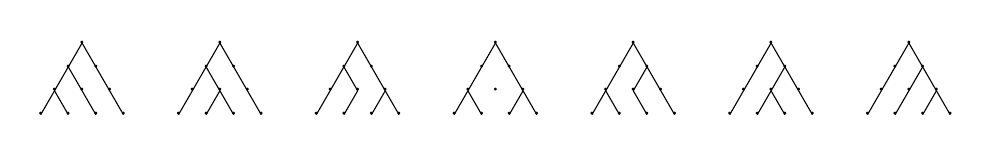
\begin{tikzpicture}[/triangle,scale=0.35]
      \def\n{3}
      \newlength{\shift}
      \setlength{\shift}{5cm}

      \foreach \k in {0,...,6} {
        \begin{scope}[xshift=\k\shift]
          \dottriangle[$\cdot$]{\n}
          \foreach \i in {1,...,\n} {
            \draw(\i-1,0) -- (\i,0);
          }
          \foreach \i in {1,...,\n} {
            \draw(\i-1,\i-1) -- (\i,\i);
          }
        \end{scope}
      }

      \begin{scope}
        \draw (1,0)--(2,1) (2,1)--(3,2) (2,0)--(3,1);
      \end{scope}

      \begin{scope}[xshift=\shift]
        \draw (1,0)--(2,1) (2,1)--(3,1) (2,1)--(3,2);
      \end{scope}

      \begin{scope}[xshift=2\shift]
        \draw (1,0)--(2,1) (2,1)--(3,1) (2,2)--(3,2);
      \end{scope}

      \begin{scope}[xshift=3\shift]
        \draw (2,0)--(3,1) (2,2)--(3,2);
      \end{scope}

      \begin{scope}[xshift=4\shift]
        \draw (1,1)--(2,1) (2,1)--(3,2) (2,0)--(3,1);
      \end{scope}

      \begin{scope}[xshift=5\shift]
        \draw (1,1)--(2,1) (2,1)--(3,2) (2,1)--(3,1);
      \end{scope}

      \begin{scope}[xshift=6\shift]
        \draw (1,1)--(2,1) (2,1)--(3,1) (2,2)--(3,2);
      \end{scope}
    \end{tikzpicture}
    \caption{The seven well formed strategies for $e=4$.}
  \end{figure}

  \begin{itemize}
  \item Right edges are \alert{$\ell$-isogeny evaluation};
  \item Left edges are \alert{multiplications by $\ell$} (about twice as expensive);
  \end{itemize}

  The best strategy can be \alert{precomputed} offline and
  \alert{hardcoded} in an embedded system.

  \begin{block}{}
    A package to explore strategies: \url{https://github.com/sidh-crypto/sidh-optimizer}.
  \end{block}
\end{frame}

%%
%%

\begin{frame}[allowframebreaks]
  \frametitle{References}

  \defbibfilter{books}{\type{book} \or \type{booklet} \or \type{thesis}
    \or \type{report} \or \type{collection} \or \type{manual}
    \or \type{periodical} \or \type{proceedings}}
  \defbibfilter{articles}{\not \(\type{book} \or \type{booklet} \or \type{thesis}
    \or \type{report} \or \type{collection} \or \type{manual}
    \or \type{periodical} \or \type{proceedings}\)}

  \beamertemplatebookbibitems
  \printbibliography[filter=books]
  \beamertemplatearticlebibitems
  \printbibliography[filter=articles]
\end{frame}

\end{document}


% LocalWords:  Isogeny abelian isogenies hyperelliptic supersingular Frobenius
% LocalWords:  isogenous


